\section{\KLUDGE 概要}

\index{HumanInterface}
HumanInterface\KLUDGE モジュールは,ハードウェアや入力デバイスを利用するための処理系に依存しないインタフェースを提供します.

\KLUDGE ほとんどの場合,HumanInterface\KLUDGE の機能はFramework\KLUDGE モジュールを介してアクセスすることになります.
\KLUDGE この場合は,後述するヒューマンインタフェースオブジェクトやデバイスの作成をユーザ自身で行う必要はありません.

\section{HumanInterface SDK}

\index{HISdk}
HumanInterface\KLUDGE モジュールのすべてのオブジェクトはSDK\KLUDGE クラス\texttt{HISdk}\KLUDGE によって管理されます.
\texttt{HISdk}\KLUDGE クラスは,プログラムの実行を通してただ1つのオブジェクトが存在するシングルトンクラスです.
\texttt{HISdk}\KLUDGE オブジェクトを作成するには以下のようにします.
\begin{sourcecode}
HISdkIf* hiSdk = HISdkIf::CreateSdk();
\end{sourcecode}
\KLUDGE 通常この操作はプログラムの初期化時に一度だけ実行します.
\KLUDGE また,Framework\KLUDGE モジュールを使用する場合はユーザが直接\texttt{HISdk}\KLUDGE を作成する必要はありません.

\section{\KLUDGE クラス階層とデータ構造}

\begin{figure}[t]
\begin{center}
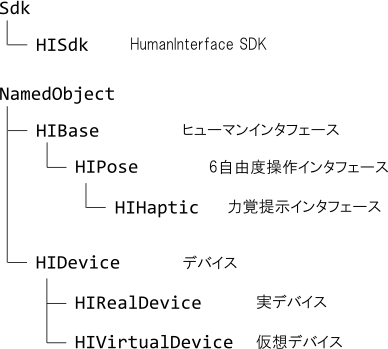
\includegraphics[width=.5\hsize]{fig/hiclass.eps}
\end{center}
\caption{HumanInterface class hierarchy}
\label{fig_hiclass}
\end{figure}

HumanInterface\KLUDGE モジュールのクラス階層をFig.\,\ref{fig_hiclass}\KLUDGE に示します.

\KLUDGE デバイスには実デバイスと仮想デバイスがあります.
\KLUDGE 実デバイスは現実のハードウェアに対応し,例えばWin32\KLUDGE マウスやあるメーカのA/D\KLUDGE 変換ボードを表す実デバイスがあります.
\KLUDGE 一方,仮想デバイスは実デバイスが提供する機能単位を表し,処理系に依存しません.
\KLUDGE 例えば,1\KLUDGE つのA/D\KLUDGE 変換ポートや抽象化されたマウスインタフェースがこれにあたります.
\KLUDGE 基本的に,初期化時を除いてはユーザは実デバイスに触れることはなく,仮想デバイスを通じてそれらの機能を利用することになります.

\KLUDGE ヒューマンインタフェースはデバイスよりも高度で抽象化された操作インタフェースを提供します.


\begin{figure}[t]
\begin{center}
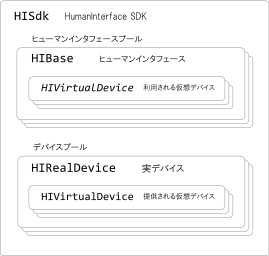
\includegraphics[width=.5\hsize]{fig/humaninterface.eps}
\end{center}
\caption{HumanInterface module data structure}
\label{fig_humaninterface}
\end{figure}

\KLUDGE 次にHumanInterface\KLUDGE モジュールのデータ構造をFig.\,\ref{fig_humaninterface}\KLUDGE に示します.
\texttt{HISdk}\KLUDGE オブジェクトはヒューマンインタフェースプールとデバイスプールを持っています.
\KLUDGE デバイスプールとは実デバイスの集まりで,それぞれの実デバイスはその機能をいくつかの仮想デバイスとして外部に提供します.

\KLUDGE デバイスの機能を使うには,
\begin{enumerate}
\item \KLUDGE 実デバイスを作成する
\item \KLUDGE 実デバイスが提供する仮想デバイスにアクセスする
\end{enumerate}
\KLUDGE という2\KLUDGE 段階の手順を踏みます.
\KLUDGE 以下にそれに関係する\texttt{HISdk}\KLUDGE の関数を紹介します.
\begin{center}
\begin{tabular}{p{.25\hsize}p{.65\hsize}}
\texttt{HISdkIf}																		\\ \midrule
\texttt{HIRealDeviceIf*}	& \texttt{AddRealDevice(const IfInfo* ii, const void* desc = NULL)} \\
\texttt{HIRealDeviceIf*}	& \texttt{FindRealDevice(const char* name)} \\
\texttt{HIRealDeviceIf*}	& \texttt{FindRealDevice(const IfInfo* ii)}
\end{tabular}
\end{center}
\texttt{AddRealDevice}\KLUDGE は型情報\texttt{ii}\KLUDGE とディスクリプタ\texttt{desc}\KLUDGE を指定して実デバイスを作成します.
\texttt{FindRealDevice}\KLUDGE は名前か型情報を指定して,既存の実デバイスを検索します.
\KLUDGE たとえば,内部でGLUT\KLUDGE を用いるキーボード・マウス実デバイスを取得するには
\begin{sourcecode}
hiSdk->FindRealDevice(DRKeyMouseGLUTIf::GetIfInfoStatic());
\end{sourcecode}
\KLUDGE とします.

\KLUDGE 仮想デバイスを取得および返却する方法には\texttt{HISdk}\KLUDGE を介する方法と\texttt{HIRealDevice}\KLUDGE を直接呼び出す方法の2\KLUDGE 通りがあります.
\begin{center}
\begin{tabular}{p{.25\hsize}p{.65\hsize}}
\texttt{HISdkIf}																							\\ \midrule
\texttt{HIVirtualDeviceIf*} & \texttt{RentVirtualDevice(const IfInfo* ii, const char* name, int portNo)}	\\
\texttt{bool}				& \texttt{ReturnVirtualDevice(HIVirtualDeviceIf* dev)}	\\
\end{tabular}
\end{center}
\texttt{RentVirtualDevice}\KLUDGE はデバイスプールをスキャンして型情報に合致した最初の仮想デバイスを返します.
\KLUDGE 実デバイスを限定したい場合は\texttt{name}\KLUDGE で実デバイス名を指定します.
\KLUDGE また,複数の仮想デバイスを提供する実デバイスもあります.
\KLUDGE この場合はポート番号\texttt{portNo}\KLUDGE で取得したい仮想デバイスを指定できます.
%
\KLUDGE デバイスの競合を防ぐために,一度取得された仮想デバイスは利用中状態になります.
\KLUDGE 利用中のデバイスは新たに取得することはできません.
\KLUDGE 使い終わったデバイスは\texttt{ReturnVirtualDevice}\KLUDGE で返却することによって再び取得可能になります.
\begin{center}
\begin{tabular}{p{.25\hsize}p{.65\hsize}}
\texttt{HIRealDeviceIf}																				\\ \midrule
\texttt{HIVirtualDeviceIf*}	& \texttt{Rent(const IfInfo* ii, const char* name, int portNo)}	\\
\texttt{bool}				& \texttt{Return(HIVirtualDeviceIf* dev)}
\end{tabular}
\end{center}
\KLUDGE こちらは実デバイスから直接取得,返却するための関数です.機能は同様です.


\section{\KLUDGE 実デバイス}

Springhead\KLUDGE ではいくつかのメーカ製のハードウェアが実デバイスとしてサポートされていますが,
\KLUDGE 処理系に強く依存する部分であるため本ドキュメントの対象外とします.
\KLUDGE 興味のある方はソースコードを見てください.

\section{\KLUDGE キーボード・マウス}
\label{sec_hi_keymouse}

\KLUDGE キーボードおよびマウスの機能は包括して1\KLUDGE つのクラスとして提供されています.
\KLUDGE キーボード・マウスの仮想デバイスは\texttt{DVKeyMouse}\KLUDGE です.
\KLUDGE 実デバイスとしてはWin32 API\KLUDGE を用いる\texttt{DRKeyMouseWin32}\KLUDGE とGLUT\KLUDGE を用いる\texttt{DRKeyMouseGLUT}\KLUDGE があります.
\KLUDGE 提供される機能に多少の差異があるので注意して下さい.

\subsection*{\KLUDGE 仮想キーコード}

Ascii\KLUDGE 外の特殊キーには処理系依存のキーコードが割り当てられています.
\KLUDGE この差を吸収するために以下のシンボルが\texttt{DVKeyCode}\KLUDGE 列挙型で定義されています.

\begin{center}
\begin{tabular}{p{.3\hsize}p{.6\hsize}}
\texttt{DVKeyCode}									\\ \midrule
\texttt{ESC}				& \KLUDGE エスケープ			\\
\texttt{F1} - \texttt{F12}	& \KLUDGE ファンクションキー	\\
\texttt{LEFT}				& \KLUDGE ←					\\
\texttt{UP}					& \KLUDGE ↑					\\
\texttt{RIGHT}				& \KLUDGE →					\\
\texttt{DOWN}				& \KLUDGE ↓					\\
\texttt{PAGE\_UP}			& Page Up				\\
\texttt{PAGE\_DOWN}			& Page Down				\\
\texttt{HOME}				& Home					\\
\texttt{END}				& End					\\
\texttt{INSERT}				& Insert				\\
\end{tabular}
\end{center}

\KLUDGE 必要に応じてシンボルが追加される可能性がありますので,完全なリストはヘッダファイルで確認してください.

\subsection*{\KLUDGE コールバック}

\texttt{DVKeyMouse}\KLUDGE からのイベントを処理するには\texttt{DVKeyMouseCallback}\KLUDGE クラスを継承し,イベントハンドラをオーバライドします.
\texttt{DVKeyMouseCallback}\KLUDGE はいくつかのヒューマンインタフェースクラスが継承しているほか,
\KLUDGE 後述するアプリケーションクラス\texttt{FWApp}\KLUDGE も継承しています.

\begin{center}
\begin{tabular}{p{.2\hsize}p{.7\hsize}}
\texttt{DVKeyMouseCallback}								\\ \midrule
\texttt{virtual bool} & \texttt{OnMouse(int button, int state, int x, int y)}		\\
\multicolumn{2}{l}{\KLUDGE マウスボタンプッシュ/\KLUDGE リリース}	\\
\\
\texttt{virtual bool} & \texttt{OnDoubleClick(int button, int x, int y)}			\\
\multicolumn{2}{l}{\KLUDGE ダブルクリック}	\\
\\
\texttt{virtual bool} & \texttt{OnMouseMove(int button, int x, int y, int zdelta)}	\\
\multicolumn{2}{l}{\KLUDGE マウスカーソル移動/\KLUDGE マウスホイール回転}	\\
\\
\texttt{virtual bool} & \texttt{OnKey(int state, int key, int x, int y)}			\\
\multicolumn{2}{l}{\KLUDGE キープッシュ/\KLUDGE リリース}	\\
\end{tabular}
\end{center}

\texttt{OnMouse}\KLUDGE はマウスボタンのプッシュあるいはリリースが生じたときに呼び出されます.
\texttt{button}\KLUDGE はイベントに関係するマウスボタンおよびいくつかの特殊キーの識別子を保持し,
\KLUDGE その値は\texttt{DVButtonMask}\KLUDGE 列挙子の値のOR\KLUDGE 結合で表現されます.
\texttt{state}\KLUDGE はマウスボタン状態変化を示し,\texttt{DVButtonSt}\KLUDGE 列挙子のいずれかの値を持ちます.
\texttt{x}\KLUDGE ,\texttt{y}\KLUDGE はイベント生成時のカーソル座標を表します.
\KLUDGE 例として,左ボタンのプッシュイベントを処理するには次のようにします.
\begin{sourcecode}
// inside your class definition ...
virtual bool OnMouse(int button, int state, int x, int y){
    if(button & DVButtonMask::LBUTTON && state == DVButtonSt::DOWN){
        // do something here
    }
}
\end{sourcecode}

\texttt{OnDoubleClick}\KLUDGE はマウスボタンのダブルクリックが生じたときに呼ばれます.
\KLUDGE 引数の定義は\texttt{OnMouse}\KLUDGE と同様です.

\texttt{OnMouseMove}\KLUDGE はマウスカーソルが移動するか,マウスホイールが回転した際に呼ばれます.
\texttt{button}\KLUDGE は直前のマウスプッシュイベントにおいて\texttt{OnMouse}\KLUDGE に渡されたのと同じ値を持ちます.
\texttt{x}, \texttt{y}\KLUDGE は移動後のカーソル座標,\texttt{zdelta}\KLUDGE はマウスカーソルの回転量です.

\texttt{OnKey}\KLUDGE はキーボードのキーがプッシュされるかリリースされた際に呼ばれます.
\texttt{state}\KLUDGE は\texttt{DVKeySt}\KLUDGE 列挙子の値を持ちます.
\texttt{key}\KLUDGE はプッシュあるいはリリースされたキーの仮想キーコードを保持します.

\KLUDGE 以下に関連する列挙子の定義を示します.

\begin{center}
\begin{tabular}{p{.3\hsize}p{.6\hsize}}
\texttt{DVButtonMask}									\\ \midrule
\texttt{LBUTTON}				& \KLUDGE 左ボタン				\\
\texttt{RBUTTON}				& \KLUDGE 右ボタン				\\
\texttt{MBUTTON}				& \KLUDGE 中ボタン				\\
\texttt{SHIFT}					& Shift\KLUDGE キー押し下げ		\\
\texttt{CONTROL}				& Ctrl\KLUDGE キー押し下げ		\\
\texttt{ALT}					& Alt\KLUDGE キー押し下げ		\\
\end{tabular}
\end{center}

\begin{center}
\begin{tabular}{p{.3\hsize}p{.6\hsize}}
\texttt{DVButtonSt}								\\ \midrule
\texttt{DOWN}			& \KLUDGE ボタンプッシュ		\\
\texttt{UP}				& \KLUDGE ボタンリリース		\\
\end{tabular}
\end{center}

\begin{center}
\begin{tabular}{p{.3\hsize}p{.6\hsize}}
\texttt{DVKeySt}								\\ \midrule
\texttt{PRESSED}		& \KLUDGE 押されている			\\
\texttt{TOGGLE\_ON}		& \KLUDGE トグルされている		\\
\end{tabular}
\end{center}

\subsection*{API\KLUDGE として提供される機能}

\KLUDGE 以下に\texttt{DVKeyMouse}\KLUDGE の関数を示します.
\begin{center}
\begin{tabular}{p{.1\hsize}p{.8\hsize}}
\texttt{DVKeyMouseIf}																		\\ \midrule
\texttt{void}	& \texttt{AddCallback(DVKeyMouseCallback*)} 	\\
\texttt{void}	& \texttt{RemoveCallback(DVKeyMouseCallback*)} 	\\
\texttt{int}	& \texttt{GetKeyState(int key)}					\\
\texttt{void}	& \texttt{GetMousePosition(int\& x, int\& y, int\& time, int count=0)}
\end{tabular}
\end{center}
\texttt{AddCallback}\KLUDGE はコールバッククラスを登録します.
\KLUDGE 一つの仮想デバイスに対して複数個のコールバックを登録できます.
\texttt{RemoveCallback}\KLUDGE は登録済のコールバッククラスを解除します.

\texttt{GetKeyState}\KLUDGE は\texttt{DVKeyCode}\KLUDGE で指定したキーの状態を\texttt{DVKeySt}\KLUDGE の値で返します.

\texttt{GetMousePosition}\KLUDGE は\texttt{count}\KLUDGE ステップ前のマウスカーソルの位置を取得するのに用います.
\KLUDGE ただし\texttt{count}\KLUDGE は$0$\KLUDGE 以上$63$\KLUDGE 以下でなければなりません.
\texttt{x}, \texttt{y}\KLUDGE にカーソル座標が,\texttt{time}\KLUDGE にタイムスタンプが格納されます.

\subsection*{\KLUDGE サポート状況に関する注意}

\KLUDGE 使用する実デバイスによっては一部の機能が提供されないので注意して下さい.

\texttt{OnMouseMove}\KLUDGE においてマウスホイールの回転量を取得するには,
\KLUDGE 実デバイスとして\texttt{DRKeyMouseWin32}\KLUDGE を使用するか,
freeglut\KLUDGE とリンクしてビルドしたSpringhead\KLUDGE 上で\texttt{DRKeyMouseGLUT}\KLUDGE を使用する必要があります.

\texttt{OnKey}\KLUDGE においてキーのトグル状態を取得するには
\KLUDGE 実デバイスとして\texttt{DRKeyMouseWin32}\KLUDGE を使用する必要があります.

\texttt{GetKeyState}\KLUDGE は\texttt{DRKeyMouseWin32}\KLUDGE でのみサポートされます.

\texttt{GetMousePosition}\KLUDGE において,タイムスタンプを取得するには\texttt{DRKeyMouseWin32}\KLUDGE を用いる必要があります.

\section{\KLUDGE ジョイスティック}

\KLUDGE ジョイスティックの仮想デバイスは\texttt{DVJoyStick}\KLUDGE です.
\KLUDGE 実デバイスとしてはGLUT\KLUDGE を用いる\texttt{DRJoyStickGLUT}\KLUDGE のみがあります.

T.B.D. 

\section{\KLUDGE トラックボール}

\begin{figure}[t]
\begin{center}
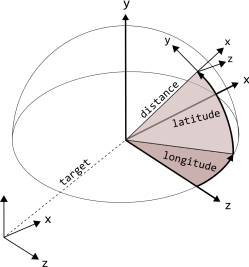
\includegraphics[width=.5\hsize]{fig/hitrackball.eps}
\end{center}
\caption{Trackball}
\label{fig_trackball}
\end{figure}

\KLUDGE トラックボールはキーボード・マウスにより並進・回転の6\KLUDGE 自由度を入力するヒューマンインタフェースです.
\KLUDGE トラックボールを使うことにより,カメラを注視点まわりに視点変更することができるようになります.

\KLUDGE トラックボールを操作する方法には,API\KLUDGE を直接呼び出す方法と,仮想マウスにコールバック登録する方法の二通りがあります.
\KLUDGE 同様に,トラックボールの状態を取得する方法にもAPI\KLUDGE 呼び出しとコールバック登録の二通りがあります.
\KLUDGE 仮想マウスとトラックボールおよびユーザプログラムの関係を\figurename\ref{fig_trackball}\KLUDGE に示します.


\subsection*{\KLUDGE 回転中心と回転角度}

\KLUDGE カメラの位置と向きは,注視点,経度角,緯度角および注視点からの距離によって決まります.

\begin{center}
\begin{tabular}{p{.15\hsize}p{.5\hsize}p{.25\hsize}}
\multicolumn{3}{l}{\texttt{HITrackballDesc}}				\\ \midrule
\texttt{Vec3f}	&	\texttt{target}			& \KLUDGE 回転中心		\\
\texttt{float}	&	\texttt{longitude}		& \KLUDGE 経度[rad]		\\
\texttt{float}	&	\texttt{latitude}		& \KLUDGE 緯度[rad]		\\
\texttt{float}	&	\texttt{distance}		& \KLUDGE 距離			\\
\end{tabular}
\end{center}

\begin{center}
\begin{tabular}{p{.15\hsize}p{.75\hsize}}
\multicolumn{2}{l}{\texttt{HITrackballIf}}									\\ \midrule
\texttt{Vec3f}	& \texttt{GetTarget()}							\\
\texttt{void} 	& \texttt{SetTarget(Vec3f)}						\\
\texttt{void} 	& \texttt{GetAngle(float\& lon, float\& lat)}	\\
\texttt{void} 	& \texttt{SetAngle(float lon, float lat)}		\\
\texttt{float} 	& \texttt{GetDistance()}						\\
\texttt{void} 	& \texttt{SetDistance(float dist)}				\\
\end{tabular}
\end{center}

\subsection*{\KLUDGE 範囲指定}

\KLUDGE 以下の機能で角度および距離に範囲制限を加えられます.

\begin{center}
\begin{tabular}{p{.15\hsize}p{.5\hsize}p{.25\hsize}}
\multicolumn{3}{l}{\texttt{HITrackballDesc}}					\\ \midrule
\texttt{Vec2f}	&	\texttt{lonRange}		& \KLUDGE 経度範囲			\\
\texttt{Vec2f}	&	\texttt{latRange}		& \KLUDGE 緯度範囲			\\
\texttt{Vec2f}	&	\texttt{distRange}		& \KLUDGE 距離範囲			\\
\end{tabular}
\end{center}

\begin{center}
\begin{tabular}{p{.15\hsize}p{.75\hsize}}
\multicolumn{2}{l}{\texttt{HITrackballIf}}									\\ \midrule
\texttt{void} 	& \texttt{GetLongitudeRange(float\& rmin, float\& rmax)}	\\
\texttt{void} 	& \texttt{SetLongitudeRange(float rmin, float rmax)}		\\
\texttt{void} 	& \texttt{GetLatitudeRange(float\& rmin, float\& rmax)}		\\
\texttt{void} 	& \texttt{SetLatitudeRange(float rmin, float rmax)}			\\
\texttt{void} 	& \texttt{GetDistanceRange(float\& rmin, float\& rmax)}		\\
\texttt{void} 	& \texttt{SetDistanceRange(float rmin, float rmax)}			\\
\end{tabular}
\end{center}

\subsection*{\KLUDGE コールバック登録}

\begin{center}
\begin{tabular}{p{.2\hsize}p{.7\hsize}}
\multicolumn{2}{l}{\texttt{HITrackballIf}}								\\ \midrule
\texttt{DVKeyMouseIf*} 	& \texttt{GetKeyMouse()}						\\
\texttt{void} 			& \texttt{SetKeyMouse(DVKeyMouseIf*)}			\\
\texttt{void} 			& \texttt{SetCallback(HITrackballCallback*)}	\\
\end{tabular}
\end{center}

\KLUDGE トラックボールをマウス操作するには\texttt{DVKeyMouse}\KLUDGE クラスにコールバック登録する必要があります.
\KLUDGE コールバック登録するには\texttt{SetKeyMouse}\KLUDGE ,登録先の仮想マウスを取得するには\texttt{GetKeyMouse}\KLUDGE を呼びます.

\KLUDGE また,ユーザプログラムがトラックボールにコールバック登録して状態変化に反応できるようにするには,
\texttt{HITrackballCallback}\KLUDGE クラスを継承し,\texttt{SetCallback}\KLUDGE 関数に渡します.
\texttt{HITrackballCallback}\KLUDGE は以下の単一の仮想関数を持ちます.
\begin{center}
\begin{tabular}{p{.2\hsize}p{.7\hsize}}
\multicolumn{2}{l}{\texttt{HITrackballCallback}}					\\ \midrule
\texttt{virtual void} 	& \texttt{OnUpdatePose(HITrackballIf* tb)}	\\
\end{tabular}
\end{center}
\texttt{OnUpdatePose}\KLUDGE はトラックボールの位置・向きに変化が生じる度に呼ばれます.
\KLUDGE 引数の\texttt{tb}\KLUDGE は呼び出し元のトラックボールを示します.

\subsection*{\KLUDGE マウスボタン割当て}

\texttt{HITrackball}\KLUDGE は内部で\texttt{DVKeyMouseCallback}\KLUDGE を継承します.
\texttt{SetKeyMouse}\KLUDGE により\texttt{DVKeyMouse}\KLUDGE にコールバック登録すると,
\KLUDGE マウスカーソルが移動するたびに\texttt{OnMouseMove}\KLUDGE イベントハンドラが呼び出され,トラックボールの内部状態が更新されます.
\KLUDGE マウス移動時のボタン状態に応じてトラックボールのどの状態が変化するかはある程度カスタマイズが可能です.
\KLUDGE 以下に関連する機能を示します.

\begin{center}
\begin{tabular}{p{.15\hsize}p{.35\hsize}p{.4\hsize}}
\multicolumn{3}{l}{\texttt{HITrackballDesc}}		\\ \midrule
\texttt{int}	& \texttt{rotMask}		& \KLUDGE 回転操作のボタン割当て		\\
\texttt{int}	& \texttt{zoomMask}		& \KLUDGE ズーム操作のボタン割当て		\\
\texttt{int}	& \texttt{trnMask}		& \KLUDGE 平行移動操作のボタン割当て	\\
\end{tabular}
\end{center}

\begin{center}
\begin{tabular}{p{.15\hsize}p{.75\hsize}}
\multicolumn{2}{l}{\texttt{HITrackballIf}}			\\ \midrule
\texttt{void} 	& \texttt{SetRotMask(int mask)}		\\
\texttt{void} 	& \texttt{SetZoomMask(int mask)}	\\
\texttt{void} 	& \texttt{SetTrnMask(int mask)}		\\
\end{tabular}
\end{center}

\texttt{rotMask}, \texttt{zoomMask}, \texttt{trnMask}\KLUDGE はそれぞれ
\KLUDGE 回転操作,ズーム操作,平行移動操作に割り当てたいマウスボタンに対応する
\texttt{OnMouseMove}\KLUDGE の\texttt{button}\KLUDGE 引数の値を表します.
\KLUDGE 以下に対応関係をまとめます.
\begin{center}
\begin{tabular}{p{.3\hsize}p{.3\hsize}p{.3\hsize}}
\toprule
\KLUDGE マウス移動方向		& \texttt{button}\KLUDGE 値		& \KLUDGE 変化量		\\ \midrule
\KLUDGE 左右				& \texttt{rotMask}		& \KLUDGE 経度			\\
\KLUDGE 上下				& \texttt{rotMask}		& \KLUDGE 緯度			\\
\KLUDGE 上下				& \texttt{zoomMask}		& \KLUDGE 距離			\\
\KLUDGE 左右				& \texttt{trnMask}		& \KLUDGE 注視点x\KLUDGE 座標	\\
\KLUDGE 上下				& \texttt{trnMask}		& \KLUDGE 注視点y\KLUDGE 座標	\\
\bottomrule
\end{tabular}
\end{center}
\KLUDGE デフォルトのボタン割当ては以下の通りです.
\begin{center}
\begin{tabular}{p{.3\hsize}p{.6\hsize}}
\texttt{rotMask}	& \texttt{LBUTTON}					\\
\texttt{zoomMask}	& \texttt{RBUTTON}					\\
\texttt{trnMask}	& \texttt{LBUTTON} + \texttt{ALT}	\\
\end{tabular}
\end{center}
\KLUDGE したがって,左ボタンドラッグで回転操作,右ボタンドラッグでズーム操作,[ALT]\KLUDGE キー+\KLUDGE 左ドラッグで平行移動となります.

\KLUDGE なお,現状ではマウスの移動方向との対応をカスタマイズすることはできません.
\KLUDGE また,マウスホイールの回転とトラックボールを連動させる機能も未実装です.

\subsection*{\KLUDGE マウス操作に対する極性と感度}

\KLUDGE マウス移動量と角度変化量,距離変化量との比例係数を下記の機能で設定できます.

\begin{center}
\begin{tabular}{p{.15\hsize}p{.35\hsize}p{.4\hsize}}
\multicolumn{3}{l}{\texttt{HITrackballDesc}}							\\ \midrule
\texttt{float}	&	\texttt{rotGain}		& \KLUDGE 回転ゲイン[rad/pixel]		\\
\texttt{float}	&	\texttt{zoomGain}		& \KLUDGE ズームゲイン[rad/pixel]	\\
\texttt{float}	&	\texttt{trnGain}		& \KLUDGE 平行移動ゲイン			\\
\end{tabular}
\end{center}

\begin{center}
\begin{tabular}{p{.15\hsize}p{.75\hsize}}
\multicolumn{2}{l}{\texttt{HITrackballIf}}									\\ \midrule
\texttt{float} 	& \texttt{GetRotGain()}			\\
\texttt{void} 	& \texttt{SetRotGain(float g)}	\\
\texttt{float} 	& \texttt{GetZoomGain()}		\\
\texttt{void} 	& \texttt{SetZoomGain(float g)}	\\
\texttt{float} 	& \texttt{GetTrnGain()}			\\
\texttt{void} 	& \texttt{SetTrnGain(float g)}	\\
\end{tabular}
\end{center}

\subsection*{\KLUDGE トラックボールで視点を動かす}

\KLUDGE トラックボールの位置と向きをカメラに反映するには,
\KLUDGE 描画処理の冒頭で以下のようにします.

\begin{sourcecode}
// given GRRenderIf* render
render->SetViewMatrix(trackball->GetAffine().inv());
\end{sourcecode}

\section{Spidar}

Spidar\KLUDGE はワイヤ駆動型の3\KLUDGE 軸・6\KLUDGE 軸力覚提示ヒューマンインタフェースです.

T.B.D. 


